\chapter{System Models}

\section{Scenarios}
Node.js based web application on a server running root and rootJS\\
\\
Webviewer launches and provides a GUI to its end user	\\
Webviewer requests data for visualization by calling rootJS\\
\indent	Node.js invokes ROOT I/O operations\\
\indent \indent		ROOT loads data and provides raw visualiztion data\\
\indent	Node.js serializes data and streams it to the web viewer\\
Webviewer receives data and renders it in the browser\\
\section{Use Cases}

\pagebreak[4]

\section{Object Models}
\begin{figure}[htb]
	\centering
	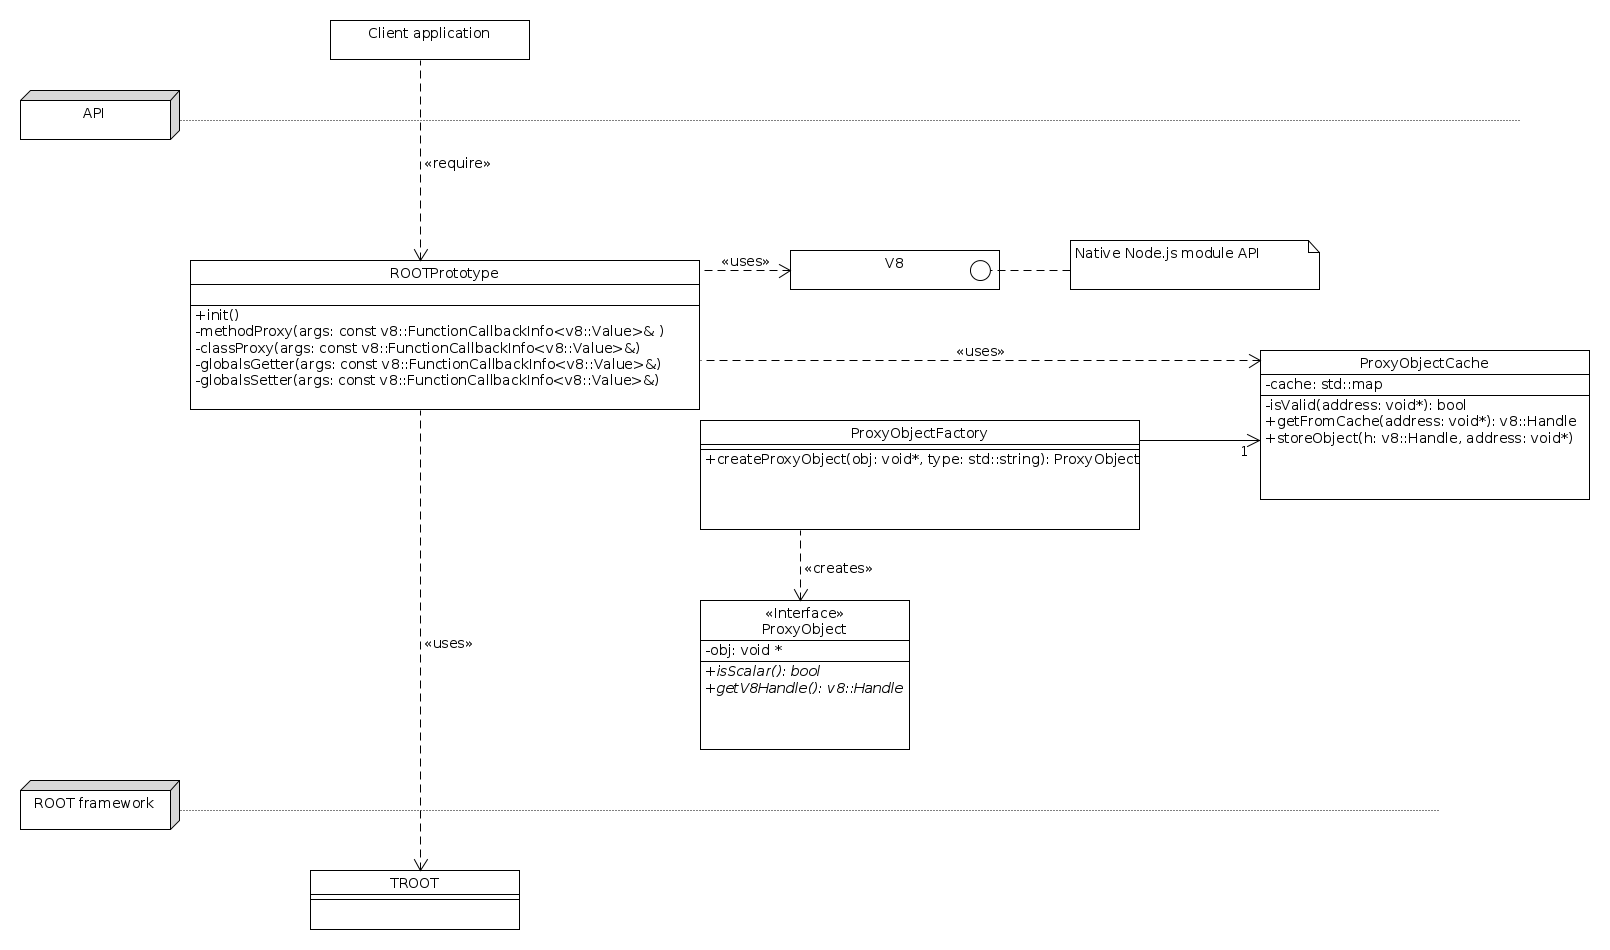
\includegraphics[width=18cm]{./latex/resources/architecture.png}
	\caption{basic architecture draft}
\end{figure}

\pagebreak[4]

\section{Dynamic Models}
\begin{figure}[htb]
	\centering
	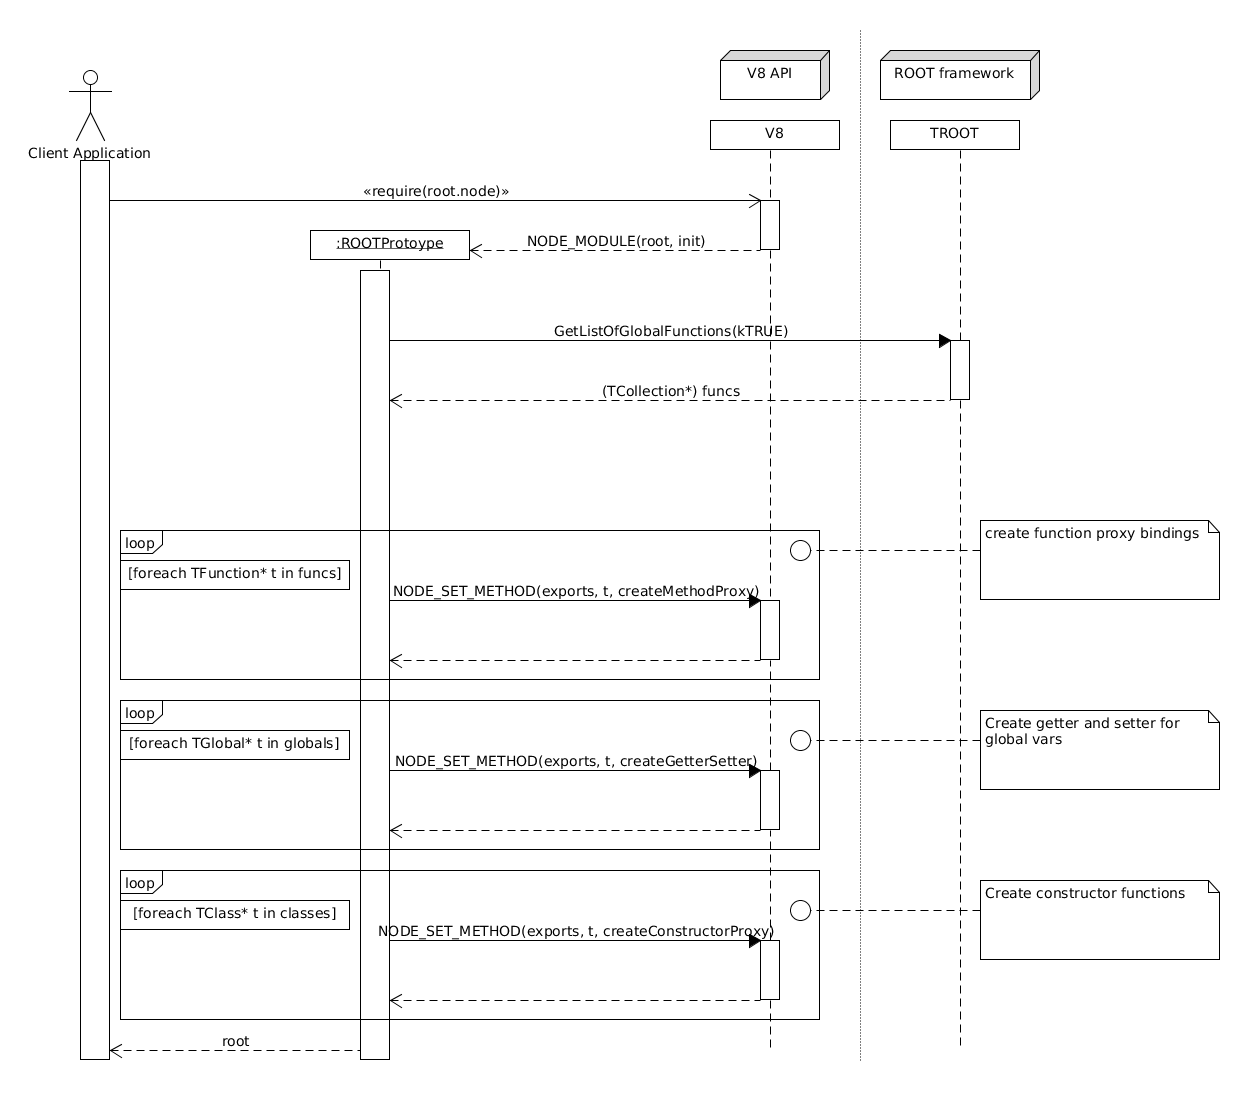
\includegraphics[width=18cm]{./latex/resources/startupSequence.png}
	\caption{startup sequence}
\end{figure}
